% !TEX root = presentation.tex

\begin{frame}
  \frametitle{Vector-Matrix Multiplication}
\center{
  \begin{tikzpicture}[ampersand replacement=\&]

    \matrix (A)[matrix of math nodes, label skeleton, left delimiter=[,right delimiter={]}]
     {
     A_{1,1} \& A_{1,2} \& A_{1,3} \& A_{1,4} \\
     };

    \matrix (B)[matrix of math nodes, label skeleton, left delimiter=[,right delimiter={]}] at (5,-0.95)
     {
     B_{1,1} \& B_{1,2} \& B_{1,3} \& B_{1,4} \& B_{1,5} \\
     B_{2,1} \& B_{2,2} \& B_{2,3} \& B_{2,4} \& B_{2,5} \\
     B_{3,1} \& B_{3,2} \& B_{3,3} \& B_{3,4} \& B_{3,5} \\
     B_{4,1} \& B_{4,2} \& B_{4,3} \& B_{4,4} \& B_{4,5} \\
     };

     \matrix (C)[matrix of math nodes, label skeleton, left delimiter=[,right delimiter={]}] at (5,-3)
      {
      C_{1,1} \& C_{1,2} \& C_{1,3} \& C_{1,4} \& C_{1,5}\\
      };

      \foreach \i in {1,...,4}
      {
      \pgfmathtruncatemacro{\ii}{\i+1}
          \onslide<\ii>{

       \foreach \j in {1,...,5}
       {
        \draw[thick] (A-1-\i.south) to [out=-90,in=135]node[visible on=<\i->, anchor=north]{} (B-\i-\j.center);

          }
        }
        }


     \end{tikzpicture}
}
\end{frame}


\begin{frame}
  \frametitle{DSP Architecture}
\scalebox{2}{
  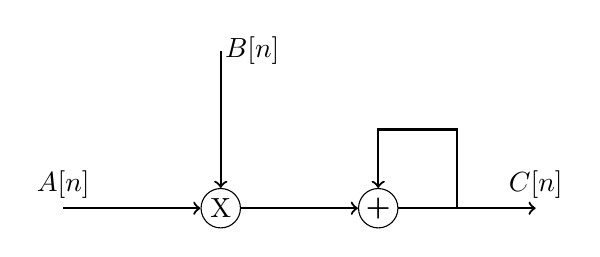
\begin{tikzpicture}
    \node (mul) at (0,0) [circle,draw=black,inner sep=0pt,minimum size=0.5cm] {X};
    \node (mac) at (2,0) [circle,draw=black,inner sep=0pt,minimum size=0.5cm] {\textbf{+}};

    \node at (-2,0.3) {$A[n]$};
    \node at (0.4,2) {$B[n]$};
    \node at (4,0.3) {$C[n]$};

    \draw[thick, ->] (-2,0) --++ (mul);
    \draw[thick, ->] (0,2) --++ (mul);
    \draw[thick, ->] (mul) -- (mac);
    \draw[thick] (mac) --++ (1,0) node (i) {};
    \draw[thick, ->] (i.center) --++ (0,1) --++ (-1,0) -- (mac);
    \draw[thick, ->] (i.center) --++ (1,0);


  \end{tikzpicture}
  }
\end{frame}
